
\chapter{维基百科中的用户分类研究}
\label{cha:user-category}

在虚拟社区中,用户是内容的创建者和分享者。社区的活力取决于用户的参与和
活跃程度,并最终影响到社区能否持续存在。
虚拟实践社区中个人的特质、参与动机、参与行为和资历的各不相同,每人的积
极程度、个人性格、表达能力和知识水平也不同,个体在社区互动中扮演的角色
不同,因而在同一虚拟社区内的用户会在社区中具有不同的行为模式,并自然分化为多
个不同的群体。

大量的研究表明,虚拟社区中总是存在着一小部分热忱的参与者和人数众多的潜
水者。积极参与的社区成员实际上介入了社区的绝大部分活动,包括内容的创
建,各类社区活动的发起和组织,以及各类日常的维护工作。Bryant曾经对英文维基
百科的活跃用户进行过调查,发现这些活跃用户所参与的工作要远远多于那些非
活跃用户,除了条目内容本身的编写外,还参与社区政策的指定,讨论社区的发
展方向,以及其他为保证社区正常运转的活动\cite{1099205}。而大多数人则只是
作为社区中的看客,很少介入到社区的活动中,尤其是那些需要投入时间和精力
的活动,例如创建新内容。这种特性已经在包括社会网络、论坛、
邮件组、维基和邮件列表等在内的各类虚拟社区中得到了验证。

通过定量分析可以发现,大部分虚拟社区的内容创建是服从幂率分布的:即一小
部分用户贡献了社区中的绝大部分内容。维基百科作为典型的以内容创建为目标
的虚拟时间社区也不例外,已经有很多研究验证了了不同语言版本的维基百科都
具有这个特点,图\ref{fig:power-law}展示了中文维
基百科中内容的贡献于用户数量之间的关系。

\begin{figure}
  \centering
 \scalebox{0.4}{ \includegraphics{02-3}}
  \caption{\small{\bf{用户数量与内容贡献的幂率分布}}}
  \label{fig:power-law}
\end{figure}

成员是虚拟社区形成和存在的基础。分清成员在虚拟社区中扮演何种角色,以及
不同类型的成员所占的比例是关系到社区能否进一步发展的重要问题。Amstrong
等提出,虚拟社区的用户是被感兴趣的话题及内容所吸引,
从而在错综复杂的网络环境中找到社区。尽管这些用户具有加入社区的潜在倾向,但还是
需要根据其兴趣及满意程度决定是否加入社区,从单纯的浏览者转变为社区用
户,参与成员的互动,直至成为生产内容的社区建设者\cite{hagel1997net}。
他们根据用户参与程度和创造的价值两个维
度将虚拟社区成员分为如下四种类型:浏览者、潜水者、贡献者
以及购买者。Adler等则根据参与形式的不同
将虚拟社区成员分为以下四种:被动者、主动者、诱导者、管理者
\cite{adler1999icp}。
%巴特勒在对基于游戏编程的MUD型虚拟社区进行多年群体动力学观察基础上,从使用动机及相关行为的角度将其用户大致分为恶作剧者(killers)、成就者(achievers)、社交者(socializes)、探索者(explorers)四类[21]。
Kozinest在研究消费虚拟社区时认为一个虚拟社区成员所属类型的确认要基于两个非独
立的因素:个人与特定的消费行为之间的关系以及个体与社区中其他成员社会关
系的强度,这两个因素是相关的。根据成员与消费活动的关系以及成员与虚拟
社区的关系两个因素,可以将虚拟社区的成员划分为四种不同的类型:浏览者、社交者、
贡献者以及内部者,如
图\ref{fig:user-type}所示\cite{kozinets2002field}:


\begin{figure}[!htp]
  \centering
  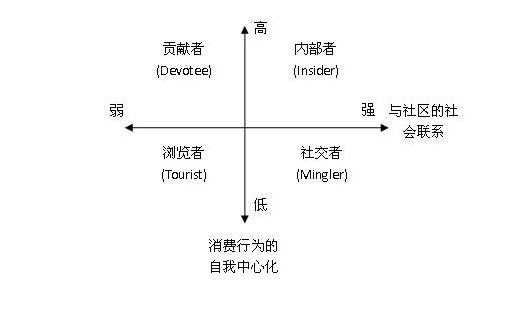
\includegraphics{users.jpg}
  \caption{\small{\textbf{虚拟社区的四种成员类型}}}
  \label{fig:user-type}
\end{figure}

杨堤雅进一步将虚拟社区成员分为了八种类别,并总结了每种类型成员的特征,
如表\ref{tab:characteristic}所示\cite{yty2000}。
\begin{table}[!htb]
  \centering \small
\caption{\small{\textbf{虚拟社区成员角色及特征}}} 
 \begin{tabular}{|c|c|c|c|c|}
    \hline
\backslashbox{特性}{角色} &参与程度&专业知识 &成员互动& 文章主要内容
\\\hline
成员领袖&高$\backslash$ 中&高&高&提供意见、分享经验\\\hline
意见呼应者&高$\backslash$ 中&中$\backslash$低&高&提供意见、分享经验
\\\hline
自我揭露者&中$\backslash$ 低&低&低&分享经验\\\hline
经验意见分享者&高$\backslash$ 中$\backslash$低$\backslash$路过&高
$\backslash$中&中&提供意见、分享经验\\\hline
查询者&低$\backslash$路过&中
$\backslash$低&中$\backslash$低&提问\\\hline
信息推广者&高$\backslash$ 中$\backslash$低$\backslash$路过&高
$\backslash$中&高$\backslash$ 中$\backslash$低&信息推广、建立关系
\\\hline
浏览者&---&低&低&无\\\hline
干扰者&低$\backslash$路过&低&低&其他\\\hline
  \end{tabular}
  
  \label{tab:characteristic}
\end{table}

用户的行为受其动机水平影响,
导致不同类型的用户有其不同的行为方式。
同时行为的结果也会影响到用户的动机水平,引起用户动机的增强或者减弱。即
使是同一种动机因素,对于不同类型的用户所起到的作用也可能是不同的。因
此,有必要对用户的类型加以区分,在此基础上分别研究动机因素对每类用户的
影响。通过对现有的文献进行分析可以发现,大部分
关于维基百科用户动机因素的研究均将社区中的所有用户视为一个整体,而并未针对
不同群体的用户特征进行专门的分析。这就使得研究的结果模糊了不同用户群体
间的区别,同时也无法提出有针对性的管理建议。本文的研究力求弥补这方面的研究空白,从用
户的知识协同动机角度出发,分析和研究用户的分类。

\section{数据处理}
\label{sec:wikimedia-data}

维基基金会大约每隔3周就会对下属所有语言版本的维基百科的数据下载备份,
形成一个时间点的归档。备份的目的除了用于灾难回复外,更重要的是为所有有
志于参与维基百科学术研究的个人和团体提供数据支持。备份的内容除了所有条
目的内容外,还包括页面链接的列表以及图片元数据等内容。备份按照包涵内容
的不同分为3种类型:
\begin{enumerate}
\item pages-articles备份。该类型的备份包含所有条目、模板和其它页面的当
  前版本,去除了条目的讨论页面和用户主页,适用于在其他地方再发布维基百
  科的内容。
\item pages-meta-current备份。提供所有页面的当前版本。
\item pages-meta-history备份。提供所有页面的所有历史版本,适合于学术研
  究。
\end{enumerate}

本研究为了分析用户的协同行为并据此为其分类,因此需要研究用户的协同贡
献,比较所有历史版本同最后版本间的内容的区别。显然,pages-meta-history备份包
含了研究所需要的全部数据。维基基金会提供了不同时段的pages-meta-history
备份,随着时间的推移,数据量显著增大。其中,最近的备份数据量在未压缩的情况下
达到了140Gb,数据的处理量非常大。为此,本研究选择了一个较小的数据集,
囊括了中文维基百科从创立至2008年8月的所有历史数据。数据集在未压缩情况
下大小为70Gb,存储格式为XML,其基本的数据结构如下:

\begin{verbatim}
<page>
    <title>Wikipedia:Upload log</title>
    <id>1</id>
    <restrictions>sysop</restrictions>
    <revision>
      <id>288633</id>
      <timestamp>2002-12-11T09:10:02Z</timestamp>
      <contributor>
        <username>Formulax</username>
        <id>3</id>
      </contributor>
      <comment>uploaded &quot;Shanghai1.jpg&quot;: 上海夜景</comment>
      <text xml:space="preserve">Below is a list of the most recent file uploads.
       .........
    </revision>
</page>
\end{verbatim}

数据由一个个<page>组成,每个page是维基百科中的一个页面(如条目页面、讨
论页面、用户页面等)。每个page包括标题、id、以及所有的历史版本等信息。
其中page的标题由两部分组成,用“:”分割开:第一部分是该page所属的命名
空间;第二部分是该page实际的标题。这样,就可以通过标题判断出该page的实
际所属类型。
通常一个page中会包括多个版本。各个版本的内容记录在<revision>标签中,包
括版本的id、该版本修订的时间、作者的相关信息、每个版本的实际文字内容和
修订备注。利用这些信息,可以得到所有的用户协同行为的量化的属性值,为下
一步分析用户行为并分类做好数据准备。

\subsection{协同用户的选择}
\label{sec:user-exclude}

本文研究的对象是维基百科社区中的用户的协同行为。社区用户应该是具有正常
行为,努力为社区发展贡献力量的用户。但是,由于维基百科社区的开放性,各
类非正常的用户不断地涌现,不仅危害了社区的正常发展,也为相应的学术研究
带来了困难。维基百科社区中不正常的用户主要包括以下几种:
\begin{enumerate}
\item 被封禁的用户。这里用户通常是在社区中有不恰当的行为,例如攻击他人、
  广告宣传以及恶意地破坏等。封禁的目的只有一个,就是防止维基百科遭到持
  续或严重破坏。对于各种不正常行为一旦确认,用户的账户即被封禁。本文认为被封禁
  的用户及其行为不应该被纳入到研究中来,因为他们的行为并不属于本文所定
  义的协同行为。%该类用户的数量为333占总数的30
\item 傀儡用户。维基百科社区规定每位用户只能拥有一个帐号,防止用户使用
  傀儡来伪造对某件事的支持度,误导他人,挑起争端,协助破坏,或回避封禁。
  除非有及特殊的原因,傀儡帐号不用来参与同社区的知识协同活动,而是进行
  伪冒、滋扰等任何违反维基百科方针的行为。傀儡也不会纳入到本文的研究范
  围。
\item 用户名不规范的用户。用户名是每一个社区用户注册后的唯一标识。维基
  百科不允许使用带有误导性、宣传性、侮辱性或破坏性的用户名;也不允许用
  户名与现实世界中各组织或团体相关,或令人混淆于具体的人或组织。一旦发现具
  有以上特征的用户名,用户可以报告至“维基百科:需要管理员注意的用户名”页
  面并附上相关的解释,管理员可于审核以后把之封禁。用户被举报
  名不意味着马上就会封禁,也就是说不会立刻出现在封禁列表中,但是历史记
  录表明绝大部分上报的用户名都受到了封禁。因此,本文排除了所有用户名不
  规范的用户。
\item 机器人用户。机器人是实际用户创建的为了完成特定目的,按照一定规则
  以自动化方式运行的账户。机器人对内容的操作极其有限,大部分机器人只能
  用于维护跨语言链接和修复重定向。除非有社群的批准,否则机器人不能用于
  拼写检查和纠正错字,以及处理繁简转换问题,尤其是对条目内容的检查。机
  器人本身并不创建任何内容,也不反应所属用户的协同行为和协同动机。本文
  的研究将机器人用户排除在外。
\item 匿名用户。关于匿名用户在维基百科社区中的作用一直是有争议的研究问
  题。就社区本身来说,尽管并不限制匿名用户的编辑,但是社区仍然鼓励用户
  注册一个账户,而非匿名编辑。维基百科认为匿名编辑的质量在本质是是存疑
  的,因此应该尽量避免。另一方面,匿名用户为识别用户带来了困难。匿名用
  户使用其IP地址作为其标识,这就意味着来自同一个IP地址的编辑可能实际上
  是由多个用户完成的,而单个用户也可能使用多个IP地址进行内容编辑。匿名
  用户本身并不是一个正常的用户状态,用户的行为也难以确认。同时,匿名用
  户本身的数量在所有用户中所占比例非常小,其贡献完全可以忽略。

\end{enumerate}

在所有的内容条目中,有一些条目也不适于纳入到研究范畴,需要从数据集中剔
除,主要包括:
\begin{enumerate}
\item 重定向页面。在维基百科中,经常会出现不同的用户针对相同的内容创建
  了不同的条目,例如“中华人民共和国”和“中国”两个条目本身的内容是一
  致的。为了避免这种情况,需要对两个条目进行合并,避免用户做重复工作,
  也使读者不会因此而产生困惑。重定向是一种特殊的页面,它提供一种运作机
  制,使得人们在输入该名称进入条目或者点击指向该名称的内部链接时,系统
  能够自动导航到重定向页面内部指定的另一相关页面中,从而实现相关页面可
  以以多个名称进行访问\footnote{http://zh.wikipedia.org/zh-cn/Help:重
    定向}。被重定向的页面将不再包含条目的实质内容,因此也就不存在用户
  的协同。
\item 消歧页和列表页。消歧义在维基百科中指消除由于不同条目拥有相同名称(一词多
  义)所引起的歧义。用户建立消歧页面,通过一些简单的注释内容消除混淆条目间的歧
  义,并引导读者链接到准确的具体的条目。列表页是为同一类别下的条目建立
  的索引式入口,如“亚洲国家列表”条目。列表页提供了该类下的所有条目的
  链接,方便导航读者。消歧页和列表页严格来说不算是合格的维基百科条目,
  而更像是方便读者的辅助性页面。另外,这两类页面的内容也常常由机器人完
  成。 
\end{enumerate}

\subsection{数据分析}
\label{sec:data-analysis}
通过对数据集的处理,提取内容条目,在去除了重定向页面、消歧页和列表页之后,共得到
205378个条目页面。所有的用户都围绕这些条目开展知识协同。社区中共有注册
用户55218名,占总用户数的$93\%$;另有数百名匿名用户和近百个机器人用户。这近六万名用户协
力完成了4592042次编辑,平均每个用户参与了77次编辑,每个条目得到了22次编辑。

利用上一章提出的计算用户协同贡献的方法,对数据进行处理。首先计算所有条
目的条目质量,计算的结果进行归一化。随后分别计算每个条目中参与用户各自
的贡献,最终可以得到每个用户在每次编辑后所做的贡献。将同一条目的编辑贡
献累加可以得到该用户为该条目所做的协同贡献,将用户所有编辑的贡献累加则
可以得到用户为整个社区所做的协同贡献。协同贡献计算完成后,本文进一步检
验了匿名用户在社区中的行为活动。匿名用户共参与了 96389个条目的知识协同活动,贡献了907763次编辑,分
别占总条目数的$46.9\%$以及总编辑次数的$19\%$。这个结果表明匿名用户似乎
是维基社区中的一股重要力量,不应该轻易舍弃。但是协同贡献的计算结果表
明,匿名用户的贡献度要远远低于注册用户的贡献度。注册用户平均每次编辑的
贡献达到了0.049,而匿名用户的平均贡献只有0.008,不及注册用户的六分之一。这
也验证了前文提到的匿名用户从总体上来说协同的质量并不高,对于社区的影响
也非常弱。
就总的协同贡献来说,匿名用户的贡献只占总量的$3\%$。因此从匿名用户的数量和对社区的
贡献两方面因素考虑,本研究不包括匿名用户的协同行为是合理的选择。

在将所有不适合
参与研究的用户从数据集中剔除,剩下的正常用户即为本文的研究对象,即维基
百科中至少参与过一次知识协同的用户。这些用户在参与社区的协同编辑过程
中逐渐分化为不同的类别,每种类别均有各自不同的行为模式和特征。但是,同
其他类型的虚拟社区不同,已有的关于用户分类的研究并不完全适合本文的研究
对象。实际上,本文所研究的用户实际上是社区中所有用户的一个子集,
即那些曾经参与过知识协同的用户。尽管这些协同用户参与维基百科社区具有相似的目的,但是仍可以根据其行
为特点划分出不同类别。因此传统的针对虚拟社区所有用户的分类并不适合本文
的研究,
需要寻找新的分类方法和维度。

首先,参与知识协同的用户已经将传统意义上的潜水者(Lurker)和浏览者
(Browser)排除在外。潜水者和浏览者均是
社区的外围成员,他们加入社区的主要目的是为了消费社区的知识产品和信息产
品,几乎没有贡献内容的行为。Yong Du分析了这两类用户产生的原因,包括:1)
认为即使自己不贡献内容也不影响社区的运行;2)希望通过加入社区进一步了
解社区的相关情况;3)不愿意与他人分享自己的知识和经验\cite{4052703}。由于维基百科的
开放性,如果一个用户试图从维基百科获取有用信息,根本就不需要进行注册,
只是单纯浏览就可以了。注册用户都是在维基百科精神的感召下,对社区已经有
了一定的了解,愿意为之贡献自己的一份力量而进行注册的。即使一部分用户注
册完之后一次编辑行为也没有,这通常是由于没有找到合适的、可以参与的条
目,或者是不熟悉界面操作等因素造成的。从广义上讲,本文所研
究的协同用户都是知识协同过程的参与者,即都是内容的生产者而非消费者。因此,本文研究的用户群并不具备这
两类用户的特征。

其次,不以协同创建内容为目的的用户也已经被排除在外。大部分虚拟社区都不可避免地存在一些不受
欢迎的用户,如破坏者和广告发布者等。这些人的存在对于社区的繁荣和发展毫
无益处,本文在数据处理过程中已经将这些用户排除。



\subsection{分类维度}
\label{sec:dimension}
用户分类可以有多种维度,每一种分类维度
都同最终研究的目标紧密相关。通过分析现有文献可以发现,很少有文献从分析用户参与
的动机角度研究用户的分类维度。
本文将用户的协同行为分为从两个角度来考察,这些角度反映了用户协同的特点,从而
最终形成分类的依据。

用户对每个条目的平均贡献是区分不同用户类型的重要维度。用户对条目的平均贡献反映了一个用户的投入程度
及其价值。条目的贡献取决于用户自身的知识水平和其将知识转化为符合维基百
科标准的内容的能力。用
户所拥有的知识越多,越是积极参与该条目的编写,那么最终在条目中所作的贡
献就越大。
不同的用户的平均贡献相差非常大。图\ref{fig:con-detri}显示了用户贡献不均衡
的分布情况。
\begin{figure}[!htb]
   \centering
 % \scalebox{0.7}{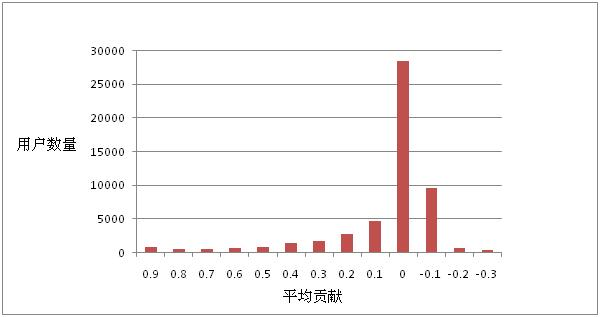
\includegraphics{con-distri.jpg}}
 % GNUPLOT: LaTeX picture
\setlength{\unitlength}{0.240900pt}
\ifx\plotpoint\undefined\newsavebox{\plotpoint}\fi
\sbox{\plotpoint}{\rule[-0.200pt]{0.400pt}{0.400pt}}%
\begin{picture}(1500,900)(0,0)
\sbox{\plotpoint}{\rule[-0.200pt]{0.400pt}{0.400pt}}%
\put(191.0,252.0){\rule[-0.200pt]{4.818pt}{0.400pt}}
\put(171,252){\makebox(0,0)[r]{5000}}
\put(1419.0,252.0){\rule[-0.200pt]{4.818pt}{0.400pt}}
\put(191.0,374.0){\rule[-0.200pt]{4.818pt}{0.400pt}}
\put(171,374){\makebox(0,0)[r]{10000}}
\put(1419.0,374.0){\rule[-0.200pt]{4.818pt}{0.400pt}}
\put(191.0,616.0){\rule[-0.200pt]{4.818pt}{0.400pt}}
\put(171,616){\makebox(0,0)[r]{20000}}
\put(1419.0,616.0){\rule[-0.200pt]{4.818pt}{0.400pt}}
\put(191.0,859.0){\rule[-0.200pt]{4.818pt}{0.400pt}}
\put(171,859){\makebox(0,0)[r]{30000}}
\put(1419.0,859.0){\rule[-0.200pt]{4.818pt}{0.400pt}}
\put(191.0,131.0){\rule[-0.200pt]{0.400pt}{4.818pt}}
\put(191,90){\makebox(0,0){-0.3}}
\put(191.0,839.0){\rule[-0.200pt]{0.400pt}{4.818pt}}
\put(287.0,131.0){\rule[-0.200pt]{0.400pt}{4.818pt}}
\put(287,90){\makebox(0,0){-0.2}}
\put(287.0,839.0){\rule[-0.200pt]{0.400pt}{4.818pt}}
\put(383.0,131.0){\rule[-0.200pt]{0.400pt}{4.818pt}}
\put(383,90){\makebox(0,0){-0.1}}
\put(383.0,839.0){\rule[-0.200pt]{0.400pt}{4.818pt}}
\put(479.0,131.0){\rule[-0.200pt]{0.400pt}{4.818pt}}
\put(479,90){\makebox(0,0){0}}
\put(479.0,839.0){\rule[-0.200pt]{0.400pt}{4.818pt}}
\put(575.0,131.0){\rule[-0.200pt]{0.400pt}{4.818pt}}
\put(575,90){\makebox(0,0){0.1}}
\put(575.0,839.0){\rule[-0.200pt]{0.400pt}{4.818pt}}
\put(671.0,131.0){\rule[-0.200pt]{0.400pt}{4.818pt}}
\put(671,90){\makebox(0,0){0.2}}
\put(671.0,839.0){\rule[-0.200pt]{0.400pt}{4.818pt}}
\put(767.0,131.0){\rule[-0.200pt]{0.400pt}{4.818pt}}
\put(767,90){\makebox(0,0){0.3}}
\put(767.0,839.0){\rule[-0.200pt]{0.400pt}{4.818pt}}
\put(863.0,131.0){\rule[-0.200pt]{0.400pt}{4.818pt}}
\put(863,90){\makebox(0,0){0.4}}
\put(863.0,839.0){\rule[-0.200pt]{0.400pt}{4.818pt}}
\put(959.0,131.0){\rule[-0.200pt]{0.400pt}{4.818pt}}
\put(959,90){\makebox(0,0){0.5}}
\put(959.0,839.0){\rule[-0.200pt]{0.400pt}{4.818pt}}
\put(1055.0,131.0){\rule[-0.200pt]{0.400pt}{4.818pt}}
\put(1055,90){\makebox(0,0){0.6}}
\put(1055.0,839.0){\rule[-0.200pt]{0.400pt}{4.818pt}}
\put(1151.0,131.0){\rule[-0.200pt]{0.400pt}{4.818pt}}
\put(1151,90){\makebox(0,0){0.7}}
\put(1151.0,839.0){\rule[-0.200pt]{0.400pt}{4.818pt}}
\put(1247.0,131.0){\rule[-0.200pt]{0.400pt}{4.818pt}}
\put(1247,90){\makebox(0,0){0.8}}
\put(1247.0,839.0){\rule[-0.200pt]{0.400pt}{4.818pt}}
\put(1343.0,131.0){\rule[-0.200pt]{0.400pt}{4.818pt}}
\put(1343,90){\makebox(0,0){0.9}}
\put(1343.0,839.0){\rule[-0.200pt]{0.400pt}{4.818pt}}
\put(1439.0,131.0){\rule[-0.200pt]{0.400pt}{4.818pt}}
\put(1439,90){\makebox(0,0){1}}
\put(1439.0,839.0){\rule[-0.200pt]{0.400pt}{4.818pt}}
\put(191.0,131.0){\rule[-0.200pt]{0.400pt}{175.375pt}}
\put(191.0,131.0){\rule[-0.200pt]{300.643pt}{0.400pt}}
\put(1439.0,131.0){\rule[-0.200pt]{0.400pt}{175.375pt}}
\put(191.0,859.0){\rule[-0.200pt]{300.643pt}{0.400pt}}
\put(30,495){\makebox(0,0){\rotatebox{90}{用户数量}}}
\put(815,29){\makebox(0,0){平均贡献}}
\put(1324.0,131.0){\rule[-0.200pt]{0.400pt}{5.059pt}}
\put(1324.0,152.0){\rule[-0.200pt]{9.154pt}{0.400pt}}
\put(1362.0,131.0){\rule[-0.200pt]{0.400pt}{5.059pt}}
\put(1324.0,131.0){\rule[-0.200pt]{9.154pt}{0.400pt}}
\put(1228.0,131.0){\rule[-0.200pt]{0.400pt}{3.613pt}}
\put(1228.0,146.0){\rule[-0.200pt]{9.154pt}{0.400pt}}
\put(1266.0,131.0){\rule[-0.200pt]{0.400pt}{3.613pt}}
\put(1228.0,131.0){\rule[-0.200pt]{9.154pt}{0.400pt}}
\put(1132.0,131.0){\rule[-0.200pt]{0.400pt}{3.132pt}}
\put(1132.0,144.0){\rule[-0.200pt]{9.154pt}{0.400pt}}
\put(1170.0,131.0){\rule[-0.200pt]{0.400pt}{3.132pt}}
\put(1132.0,131.0){\rule[-0.200pt]{9.154pt}{0.400pt}}
\put(1036.0,131.0){\rule[-0.200pt]{0.400pt}{3.613pt}}
\put(1036.0,146.0){\rule[-0.200pt]{9.154pt}{0.400pt}}
\put(1074.0,131.0){\rule[-0.200pt]{0.400pt}{3.613pt}}
\put(1036.0,131.0){\rule[-0.200pt]{9.154pt}{0.400pt}}
\put(940.0,131.0){\rule[-0.200pt]{0.400pt}{4.818pt}}
\put(940.0,151.0){\rule[-0.200pt]{9.154pt}{0.400pt}}
\put(978.0,131.0){\rule[-0.200pt]{0.400pt}{4.818pt}}
\put(940.0,131.0){\rule[-0.200pt]{9.154pt}{0.400pt}}
\put(844.0,131.0){\rule[-0.200pt]{0.400pt}{8.431pt}}
\put(844.0,166.0){\rule[-0.200pt]{9.154pt}{0.400pt}}
\put(882.0,131.0){\rule[-0.200pt]{0.400pt}{8.431pt}}
\put(844.0,131.0){\rule[-0.200pt]{9.154pt}{0.400pt}}
\put(748.0,131.0){\rule[-0.200pt]{0.400pt}{10.600pt}}
\put(748.0,175.0){\rule[-0.200pt]{9.154pt}{0.400pt}}
\put(786.0,131.0){\rule[-0.200pt]{0.400pt}{10.600pt}}
\put(748.0,131.0){\rule[-0.200pt]{9.154pt}{0.400pt}}
\put(652.0,131.0){\rule[-0.200pt]{0.400pt}{16.622pt}}
\put(652.0,200.0){\rule[-0.200pt]{9.154pt}{0.400pt}}
\put(690.0,131.0){\rule[-0.200pt]{0.400pt}{16.622pt}}
\put(652.0,131.0){\rule[-0.200pt]{9.154pt}{0.400pt}}
\put(556.0,131.0){\rule[-0.200pt]{0.400pt}{27.222pt}}
\put(556.0,244.0){\rule[-0.200pt]{9.154pt}{0.400pt}}
\put(594.0,131.0){\rule[-0.200pt]{0.400pt}{27.222pt}}
\put(556.0,131.0){\rule[-0.200pt]{9.154pt}{0.400pt}}
\put(460.0,131.0){\rule[-0.200pt]{0.400pt}{166.221pt}}
\put(460.0,821.0){\rule[-0.200pt]{9.154pt}{0.400pt}}
\put(498.0,131.0){\rule[-0.200pt]{0.400pt}{166.221pt}}
\put(460.0,131.0){\rule[-0.200pt]{9.154pt}{0.400pt}}
\put(364.0,131.0){\rule[-0.200pt]{0.400pt}{56.371pt}}
\put(364.0,365.0){\rule[-0.200pt]{9.154pt}{0.400pt}}
\put(402.0,131.0){\rule[-0.200pt]{0.400pt}{56.371pt}}
\put(364.0,131.0){\rule[-0.200pt]{9.154pt}{0.400pt}}
\put(268.0,131.0){\rule[-0.200pt]{0.400pt}{4.095pt}}
\put(268.0,148.0){\rule[-0.200pt]{9.154pt}{0.400pt}}
\put(306.0,131.0){\rule[-0.200pt]{0.400pt}{4.095pt}}
\put(268.0,131.0){\rule[-0.200pt]{9.154pt}{0.400pt}}
\put(191.0,131.0){\rule[-0.200pt]{0.400pt}{2.168pt}}
\put(191.0,140.0){\rule[-0.200pt]{4.577pt}{0.400pt}}
\put(210.0,131.0){\rule[-0.200pt]{0.400pt}{2.168pt}}
\put(191.0,131.0){\rule[-0.200pt]{4.577pt}{0.400pt}}
\put(191.0,131.0){\rule[-0.200pt]{0.400pt}{175.375pt}}
\put(191.0,131.0){\rule[-0.200pt]{300.643pt}{0.400pt}}
\put(1439.0,131.0){\rule[-0.200pt]{0.400pt}{175.375pt}}
\put(191.0,859.0){\rule[-0.200pt]{300.643pt}{0.400pt}}
\end{picture}
  
\caption{\small{\textbf{用户平均贡献分布}}}
 \label{fig:con-detri}
\end{figure}

图中显示了每个贡献度区间内的用户数量。可以看到贡献度的分布明显可以分为
几个部分。从0.9至0.5这个区间可以看出用户分布非常均匀,几乎每个区间段的
用户数量差别都不大。从0.5-0.1区间,用户数量开始稳步提升。在区间
[0.1,-0.1]之间用户数量暴涨,在这个区间的用户数达到了总用户数的$69\%$。
随后用户数量迅速减少。

不同区段的用户,其行为特点也非常鲜明。对于平均贡献大于0.5的用户来说,这意味
着一个条目中有超过一半的内容是由该用户贡献的。称这名用户为该条目的主导
者毫不为过。这类用户除了亲自编写内容外,往往还会负责引领条目的编写方
向,规划内容的结构等,是组织条目编写的积极的带头人。对于平均贡献在0.1
至0.5这个区间的用户来说,他们尽管在知识协同中不占据主导力量,却是
整个协同过程中不可或缺的中坚力量。毕竟条目带头人的群体只占总用户数量的
$6.6\%$,面对数量如此众多的条目,仅靠这一小部分人是无法完成的。这类用
户是前一类用户积极的追随者和稳定的协同实践者,按照条目编辑的预定目标,最大程度地贡献
自己的力量。最后一类用户是整个用户群体的低端用户,他们的平均贡献不超过
0.1。这意味着他们在条目编辑过程中所起的作用微不足道。甚至,平均贡献为
负值的用户占到了总用户数的$20.5\%$。从数值上看,很难说这个用户群体究竟
对维基百科社区起到了关键作用。但是,这个数量庞大的群体却是社区存在的坚
实基础。首先,所有的高级用户均产生于这个用户群体。任何的高级用户必然要经历一个
从初级用户到高级用户的过程,在这个过程中不断增加对社区的了解,不断提升
自己的技能和经验,最终才能带领其他用户共同建设一个繁荣的社区。只有拥有
数量庞大的初级用户群体,才会不断地产生更多的高级用户。其次,这些初级用
户所参与的工作大部分是维护性的工作,如修正条目中的错别字,改进内容的表
达方式,补充内容来源等工作。这些工作虽小,但是对于改进读者的阅读体验却有很大帮
助。因此,尽管这个用户群短期内对社区发展的影响很小,但是社区仍应将其视
为社区发展的重要资源。

另一个分类维度是用户参与编辑的条目数量。这个角度反映了用户的参与和活跃
程度。积极的用户往往不满足于参与有限的几个条目编辑中去,而是希望能尽可能地
为更多的条目贡献自己的力量。用户越是活跃,越
是积极参与,那么该用户所涉及到的条目也就越多。

同用户的平均贡献类似,用户参与的条目数量的分布也是极为不均衡。绝大部分
在其加入社区的整个生命周期内只参与了一、两个条目的协同。图\ref{fig:user-entry-1}显示了参与
条目数量在10以内的用户分布。
\begin{figure}[htb]
  \centering
% \scalebox{0.68}{ 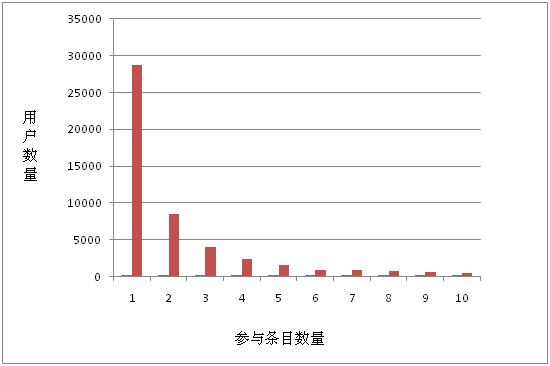
\includegraphics{user-entry-1.jpg}}
 % GNUPLOT: LaTeX picture
\setlength{\unitlength}{0.240900pt}
\ifx\plotpoint\undefined\newsavebox{\plotpoint}\fi
\begin{picture}(1500,900)(0,0)
\sbox{\plotpoint}{\rule[-0.200pt]{0.400pt}{0.400pt}}%
\put(191.0,252.0){\rule[-0.200pt]{4.818pt}{0.400pt}}
\put(171,252){\makebox(0,0)[r]{5000}}
\put(1419.0,252.0){\rule[-0.200pt]{4.818pt}{0.400pt}}
\put(191.0,374.0){\rule[-0.200pt]{4.818pt}{0.400pt}}
\put(171,374){\makebox(0,0)[r]{10000}}
\put(1419.0,374.0){\rule[-0.200pt]{4.818pt}{0.400pt}}
\put(191.0,616.0){\rule[-0.200pt]{4.818pt}{0.400pt}}
\put(171,616){\makebox(0,0)[r]{20000}}
\put(1419.0,616.0){\rule[-0.200pt]{4.818pt}{0.400pt}}
\put(191.0,859.0){\rule[-0.200pt]{4.818pt}{0.400pt}}
\put(171,859){\makebox(0,0)[r]{30000}}
\put(1419.0,859.0){\rule[-0.200pt]{4.818pt}{0.400pt}}
\put(191.0,131.0){\rule[-0.200pt]{0.400pt}{4.818pt}}
\put(191,90){\makebox(0,0){0}}
\put(191.0,839.0){\rule[-0.200pt]{0.400pt}{4.818pt}}
\put(304.0,131.0){\rule[-0.200pt]{0.400pt}{4.818pt}}
\put(304,90){\makebox(0,0){1}}
\put(304.0,839.0){\rule[-0.200pt]{0.400pt}{4.818pt}}
\put(418.0,131.0){\rule[-0.200pt]{0.400pt}{4.818pt}}
\put(418,90){\makebox(0,0){2}}
\put(418.0,839.0){\rule[-0.200pt]{0.400pt}{4.818pt}}
\put(531.0,131.0){\rule[-0.200pt]{0.400pt}{4.818pt}}
\put(531,90){\makebox(0,0){3}}
\put(531.0,839.0){\rule[-0.200pt]{0.400pt}{4.818pt}}
\put(645.0,131.0){\rule[-0.200pt]{0.400pt}{4.818pt}}
\put(645,90){\makebox(0,0){4}}
\put(645.0,839.0){\rule[-0.200pt]{0.400pt}{4.818pt}}
\put(758.0,131.0){\rule[-0.200pt]{0.400pt}{4.818pt}}
\put(758,90){\makebox(0,0){5}}
\put(758.0,839.0){\rule[-0.200pt]{0.400pt}{4.818pt}}
\put(872.0,131.0){\rule[-0.200pt]{0.400pt}{4.818pt}}
\put(872,90){\makebox(0,0){6}}
\put(872.0,839.0){\rule[-0.200pt]{0.400pt}{4.818pt}}
\put(985.0,131.0){\rule[-0.200pt]{0.400pt}{4.818pt}}
\put(985,90){\makebox(0,0){7}}
\put(985.0,839.0){\rule[-0.200pt]{0.400pt}{4.818pt}}
\put(1099.0,131.0){\rule[-0.200pt]{0.400pt}{4.818pt}}
\put(1099,90){\makebox(0,0){8}}
\put(1099.0,839.0){\rule[-0.200pt]{0.400pt}{4.818pt}}
\put(1212.0,131.0){\rule[-0.200pt]{0.400pt}{4.818pt}}
\put(1212,90){\makebox(0,0){9}}
\put(1212.0,839.0){\rule[-0.200pt]{0.400pt}{4.818pt}}
\put(1326.0,131.0){\rule[-0.200pt]{0.400pt}{4.818pt}}
\put(1326,90){\makebox(0,0){10}}
\put(1326.0,839.0){\rule[-0.200pt]{0.400pt}{4.818pt}}
\put(1439.0,131.0){\rule[-0.200pt]{0.400pt}{4.818pt}}
\put(1439,90){\makebox(0,0){11}}
\put(1439.0,839.0){\rule[-0.200pt]{0.400pt}{4.818pt}}
\put(191.0,131.0){\rule[-0.200pt]{0.400pt}{175.375pt}}
\put(191.0,131.0){\rule[-0.200pt]{300.643pt}{0.400pt}}
\put(1439.0,131.0){\rule[-0.200pt]{0.400pt}{175.375pt}}
\put(191.0,859.0){\rule[-0.200pt]{300.643pt}{0.400pt}}
\put(30,495){\makebox(0,0){\rotatebox{90}{用户数量}}}
\put(815,29){\makebox(0,0){参与条目}}
\put(287.0,131.0){\rule[-0.200pt]{0.400pt}{168.148pt}}
\put(287.0,829.0){\rule[-0.200pt]{8.191pt}{0.400pt}}
\put(321.0,131.0){\rule[-0.200pt]{0.400pt}{168.148pt}}
\put(287.0,131.0){\rule[-0.200pt]{8.191pt}{0.400pt}}
\put(401.0,131.0){\rule[-0.200pt]{0.400pt}{49.625pt}}
\put(401.0,337.0){\rule[-0.200pt]{8.191pt}{0.400pt}}
\put(435.0,131.0){\rule[-0.200pt]{0.400pt}{49.625pt}}
\put(401.0,131.0){\rule[-0.200pt]{8.191pt}{0.400pt}}
\put(514.0,131.0){\rule[-0.200pt]{0.400pt}{23.126pt}}
\put(514.0,227.0){\rule[-0.200pt]{8.191pt}{0.400pt}}
\put(548.0,131.0){\rule[-0.200pt]{0.400pt}{23.126pt}}
\put(514.0,131.0){\rule[-0.200pt]{8.191pt}{0.400pt}}
\put(628.0,131.0){\rule[-0.200pt]{0.400pt}{13.731pt}}
\put(628.0,188.0){\rule[-0.200pt]{8.191pt}{0.400pt}}
\put(662.0,131.0){\rule[-0.200pt]{0.400pt}{13.731pt}}
\put(628.0,131.0){\rule[-0.200pt]{8.191pt}{0.400pt}}
\put(741.0,131.0){\rule[-0.200pt]{0.400pt}{9.154pt}}
\put(741.0,169.0){\rule[-0.200pt]{8.191pt}{0.400pt}}
\put(775.0,131.0){\rule[-0.200pt]{0.400pt}{9.154pt}}
\put(741.0,131.0){\rule[-0.200pt]{8.191pt}{0.400pt}}
\put(855.0,131.0){\rule[-0.200pt]{0.400pt}{5.059pt}}
\put(855.0,152.0){\rule[-0.200pt]{8.191pt}{0.400pt}}
\put(889.0,131.0){\rule[-0.200pt]{0.400pt}{5.059pt}}
\put(855.0,131.0){\rule[-0.200pt]{8.191pt}{0.400pt}}
\put(968.0,131.0){\rule[-0.200pt]{0.400pt}{5.059pt}}
\put(968.0,152.0){\rule[-0.200pt]{8.191pt}{0.400pt}}
\put(1002.0,131.0){\rule[-0.200pt]{0.400pt}{5.059pt}}
\put(968.0,131.0){\rule[-0.200pt]{8.191pt}{0.400pt}}
\put(1082.0,131.0){\rule[-0.200pt]{0.400pt}{4.095pt}}
\put(1082.0,148.0){\rule[-0.200pt]{8.191pt}{0.400pt}}
\put(1116.0,131.0){\rule[-0.200pt]{0.400pt}{4.095pt}}
\put(1082.0,131.0){\rule[-0.200pt]{8.191pt}{0.400pt}}
\put(1195.0,131.0){\rule[-0.200pt]{0.400pt}{3.132pt}}
\put(1195.0,144.0){\rule[-0.200pt]{8.191pt}{0.400pt}}
\put(1229.0,131.0){\rule[-0.200pt]{0.400pt}{3.132pt}}
\put(1195.0,131.0){\rule[-0.200pt]{8.191pt}{0.400pt}}
\put(1309.0,131.0){\rule[-0.200pt]{0.400pt}{2.650pt}}
\put(1309.0,142.0){\rule[-0.200pt]{8.191pt}{0.400pt}}
\put(1343.0,131.0){\rule[-0.200pt]{0.400pt}{2.650pt}}
\put(1309.0,131.0){\rule[-0.200pt]{8.191pt}{0.400pt}}
\put(191.0,131.0){\rule[-0.200pt]{0.400pt}{175.375pt}}
\put(191.0,131.0){\rule[-0.200pt]{300.643pt}{0.400pt}}
\put(1439.0,131.0){\rule[-0.200pt]{0.400pt}{175.375pt}}
\put(191.0,859.0){\rule[-0.200pt]{300.643pt}{0.400pt}}
\end{picture}

  \caption{\small{\textbf{用户参与的条目数量}}}
  \label{fig:user-entry-1}
\end{figure}

从图中可以看出,只参与了一个条目编写的用户数量达到了28749人,占总
用户数量的$52\%$。即有超过一半的用户处于这种极度不活跃的状态。而编辑条目数在5个以下的用户数共计45187人,占总用户数
量的$81.83\%$。这一部分用户可以视为社区中的不活跃人群,他们因为各种原
因没能找到发挥自己才能的条目,成为了沉默者。社区流失的成员大部分来自于
这个群体。从用户的分布数量看,编辑条目数量在1--5之间的用户数量从最大值
28749人急剧减少,随后,人数呈缓慢的下降趋势,由于数值太小,难以看出分
布随后的变化趋势。图\ref{fig:user-entry-2}进一步显示了较活跃的用户数量
的分布。
\begin{figure}[htb]
  \centering
% \scalebox{0.68}{ 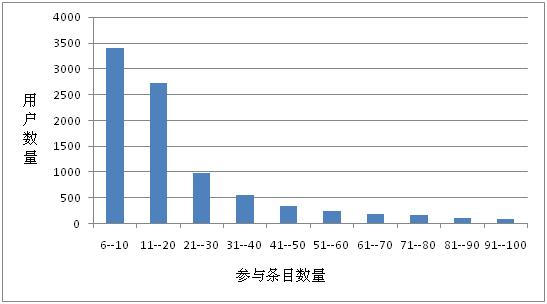
\includegraphics{user-entry-2.jpg}}
  % GNUPLOT: LaTeX picture
\setlength{\unitlength}{0.240900pt}
\ifx\plotpoint\undefined\newsavebox{\plotpoint}\fi
\begin{picture}(1500,900)(0,0)
\sbox{\plotpoint}{\rule[-0.200pt]{0.400pt}{0.400pt}}%
\put(171.0,235.0){\rule[-0.200pt]{4.818pt}{0.400pt}}
\put(151,235){\makebox(0,0)[r]{500}}
\put(1419.0,235.0){\rule[-0.200pt]{4.818pt}{0.400pt}}
\put(171.0,339.0){\rule[-0.200pt]{4.818pt}{0.400pt}}
\put(151,339){\makebox(0,0)[r]{1000}}
\put(1419.0,339.0){\rule[-0.200pt]{4.818pt}{0.400pt}}
\put(171.0,547.0){\rule[-0.200pt]{4.818pt}{0.400pt}}
\put(151,547){\makebox(0,0)[r]{2000}}
\put(1419.0,547.0){\rule[-0.200pt]{4.818pt}{0.400pt}}
\put(171.0,859.0){\rule[-0.200pt]{4.818pt}{0.400pt}}
\put(151,859){\makebox(0,0)[r]{3500}}
\put(1419.0,859.0){\rule[-0.200pt]{4.818pt}{0.400pt}}
\put(286.0,131.0){\rule[-0.200pt]{0.400pt}{4.818pt}}
\put(286,90){\makebox(0,0){6-10}}
\put(286.0,839.0){\rule[-0.200pt]{0.400pt}{4.818pt}}
\put(402.0,131.0){\rule[-0.200pt]{0.400pt}{4.818pt}}
\put(402,90){\makebox(0,0){20  }}
\put(402.0,839.0){\rule[-0.200pt]{0.400pt}{4.818pt}}
\put(517.0,131.0){\rule[-0.200pt]{0.400pt}{4.818pt}}
\put(517,90){\makebox(0,0){30\ }}
\put(517.0,839.0){\rule[-0.200pt]{0.400pt}{4.818pt}}
\put(632.0,131.0){\rule[-0.200pt]{0.400pt}{4.818pt}}
\put(632,90){\makebox(0,0){40  }}
\put(632.0,839.0){\rule[-0.200pt]{0.400pt}{4.818pt}}
\put(747.0,131.0){\rule[-0.200pt]{0.400pt}{4.818pt}}
\put(747,90){\makebox(0,0){50  }}
\put(747.0,839.0){\rule[-0.200pt]{0.400pt}{4.818pt}}
\put(863.0,131.0){\rule[-0.200pt]{0.400pt}{4.818pt}}
\put(863,90){\makebox(0,0){60  }}
\put(863.0,839.0){\rule[-0.200pt]{0.400pt}{4.818pt}}
\put(978.0,131.0){\rule[-0.200pt]{0.400pt}{4.818pt}}
\put(978,90){\makebox(0,0){70  }}
\put(978.0,839.0){\rule[-0.200pt]{0.400pt}{4.818pt}}
\put(1093.0,131.0){\rule[-0.200pt]{0.400pt}{4.818pt}}
\put(1093,90){\makebox(0,0){80  }}
\put(1093.0,839.0){\rule[-0.200pt]{0.400pt}{4.818pt}}
\put(1208.0,131.0){\rule[-0.200pt]{0.400pt}{4.818pt}}
\put(1208,90){\makebox(0,0){90  }}
\put(1208.0,839.0){\rule[-0.200pt]{0.400pt}{4.818pt}}
\put(1324.0,131.0){\rule[-0.200pt]{0.400pt}{4.818pt}}
\put(1324,90){\makebox(0,0){>90}}
\put(1324.0,839.0){\rule[-0.200pt]{0.400pt}{4.818pt}}
\put(1439.0,131.0){\rule[-0.200pt]{0.400pt}{4.818pt}}
\put(1439,90){\makebox(0,0){ }}
\put(1439.0,839.0){\rule[-0.200pt]{0.400pt}{4.818pt}}
\put(171.0,131.0){\rule[-0.200pt]{0.400pt}{175.375pt}}
\put(171.0,131.0){\rule[-0.200pt]{305.461pt}{0.400pt}}
\put(1439.0,131.0){\rule[-0.200pt]{0.400pt}{175.375pt}}
\put(171.0,859.0){\rule[-0.200pt]{305.461pt}{0.400pt}}
\put(30,495){\makebox(0,0){\rotatebox{90}{用户数量}}}
\put(805,29){\makebox(0,0){参与条目}}
\put(269.0,131.0){\rule[-0.200pt]{0.400pt}{170.316pt}}
\put(269.0,838.0){\rule[-0.200pt]{8.431pt}{0.400pt}}
\put(304.0,131.0){\rule[-0.200pt]{0.400pt}{170.316pt}}
\put(269.0,131.0){\rule[-0.200pt]{8.431pt}{0.400pt}}
\put(384.0,131.0){\rule[-0.200pt]{0.400pt}{136.349pt}}
\put(384.0,697.0){\rule[-0.200pt]{8.431pt}{0.400pt}}
\put(419.0,131.0){\rule[-0.200pt]{0.400pt}{136.349pt}}
\put(384.0,131.0){\rule[-0.200pt]{8.431pt}{0.400pt}}
\put(500.0,131.0){\rule[-0.200pt]{0.400pt}{49.144pt}}
\put(500.0,335.0){\rule[-0.200pt]{8.191pt}{0.400pt}}
\put(534.0,131.0){\rule[-0.200pt]{0.400pt}{49.144pt}}
\put(500.0,131.0){\rule[-0.200pt]{8.191pt}{0.400pt}}
\put(615.0,131.0){\rule[-0.200pt]{0.400pt}{27.222pt}}
\put(615.0,244.0){\rule[-0.200pt]{8.191pt}{0.400pt}}
\put(649.0,131.0){\rule[-0.200pt]{0.400pt}{27.222pt}}
\put(615.0,131.0){\rule[-0.200pt]{8.191pt}{0.400pt}}
\put(730.0,131.0){\rule[-0.200pt]{0.400pt}{17.104pt}}
\put(730.0,202.0){\rule[-0.200pt]{8.431pt}{0.400pt}}
\put(765.0,131.0){\rule[-0.200pt]{0.400pt}{17.104pt}}
\put(730.0,131.0){\rule[-0.200pt]{8.431pt}{0.400pt}}
\put(845.0,131.0){\rule[-0.200pt]{0.400pt}{12.045pt}}
\put(845.0,181.0){\rule[-0.200pt]{8.431pt}{0.400pt}}
\put(880.0,131.0){\rule[-0.200pt]{0.400pt}{12.045pt}}
\put(845.0,131.0){\rule[-0.200pt]{8.431pt}{0.400pt}}
\put(961.0,131.0){\rule[-0.200pt]{0.400pt}{9.636pt}}
\put(961.0,171.0){\rule[-0.200pt]{8.191pt}{0.400pt}}
\put(995.0,131.0){\rule[-0.200pt]{0.400pt}{9.636pt}}
\put(961.0,131.0){\rule[-0.200pt]{8.191pt}{0.400pt}}
\put(1076.0,131.0){\rule[-0.200pt]{0.400pt}{7.950pt}}
\put(1076.0,164.0){\rule[-0.200pt]{8.191pt}{0.400pt}}
\put(1110.0,131.0){\rule[-0.200pt]{0.400pt}{7.950pt}}
\put(1076.0,131.0){\rule[-0.200pt]{8.191pt}{0.400pt}}
\put(1191.0,131.0){\rule[-0.200pt]{0.400pt}{5.782pt}}
\put(1191.0,155.0){\rule[-0.200pt]{8.431pt}{0.400pt}}
\put(1226.0,131.0){\rule[-0.200pt]{0.400pt}{5.782pt}}
\put(1191.0,131.0){\rule[-0.200pt]{8.431pt}{0.400pt}}
\put(1306.0,131.0){\rule[-0.200pt]{0.400pt}{4.336pt}}
\put(1306.0,149.0){\rule[-0.200pt]{8.431pt}{0.400pt}}
\put(1341.0,131.0){\rule[-0.200pt]{0.400pt}{4.336pt}}
\put(1306.0,131.0){\rule[-0.200pt]{8.431pt}{0.400pt}}
\put(171.0,131.0){\rule[-0.200pt]{0.400pt}{175.375pt}}
\put(171.0,131.0){\rule[-0.200pt]{305.461pt}{0.400pt}}
\put(1439.0,131.0){\rule[-0.200pt]{0.400pt}{175.375pt}}
\put(171.0,859.0){\rule[-0.200pt]{305.461pt}{0.400pt}}
\end{picture}

 \caption{\small{用户参与的条目数量(2)}}
  \label{fig:user-entry-2}
\end{figure}

图\ref{fig:user-entry-2}也表现出类似的用户分布。用户数量先是显著下降,
当到达51--60这个区间段后开始平缓下降。可以认为从这个区间段开始,用户表
现出了非常显著和活跃的协同行为。当一个用户参与条目的数量超过了50,表明
该用户已经完全熟悉并掌握了社区的基本规则,确立了自身的定位,并以一种非
常积极的态度参与到社区的协同活动中来。这一群体的用户是维基精神的积极践
行者。尽管他们可能不具有很多的专业知识,不能引领每一个条目的发展方向,
但是他们尽可能地发挥自身的优势,以巨大的热情为社区做出自己的贡献。在这
类用户中还存在着是一些“超人”用户:有10个用户参与的条目数量超过了
10000,其中参与条目最多的用户达到了23991个条目。正是这类活跃用户的努力
繁荣了整个社区。第三类用户是处于上述两
类用户之间的“中间用户”。这类用户逐渐从不活跃的状态向活跃状态转变,开始有
意识地寻找一些自己关心或是感兴趣的条目,试图从中发现可以贡献自身知识的
机会。另一方面,这一类用户由于时间、精力等方面的因素,没能象活跃用户那
样全情投入。尽管如此,由于人数上的优势(约为活跃用户的4倍),这类用户
仍然是社区繁荣的可靠力量。

通过以上分析的两个分类维度以及每个分类维度下的分类原则,最终可以得到适
用于分析用户协同行为及其特征的分类法。所有的用户按照该分类法都会分到一
个恰当的类别中去,分类的结果如表\ref{tab:category}所示:
\begin{table}[htb]
  \centering
 \small
 \caption{\small{用户分类结果}}
  \begin{tabular}{|c|c|c|c|c|}
\hline
    分类&条目平均贡献&参与条目数量&人数&百分比\\\hline
    分类1&高&高&61&$0.11\%$\\\hline
    分类2&高&中&224&$0.41\%$\\\hline
    分类3&高&低&3182&$5.76\%$\\\hline
    分类4&中&高&1027&$1.86\%$\\\hline
    分类5&中&中&2835&$5.13\%$\\\hline
    分类6&中&低&6866&$12.43\%$\\\hline
    分类7&低&高&1044&$1.89\%$\\\hline
    分类8&低&中&4839&$8.76\%$\\\hline
    分类9&低&低&35139&$63.64\%$\\\hline
  \end{tabular}
 
  \label{tab:category}
\end{table}

初始的分类结果形成了9个分类,并且不同分类间用户数量相差非常大。由于本
研究的目的是考察不同类型的用户参与知识协同的动机因素,因此形成的用户分
类应该符合两个特点:1)分类之间的界限明显,分类应该突出突出本类别用户的明
显特点;2)分类应该与时间关联较小。用户由于加入社区在时间上有早晚,因此用
户特征会随时间变化,从一种类型的用户转变为另一种类型的用户。如果分类本
身与时间的关联度很高,则意味着该类别的用户转换速度非常快,该分类很可能
只是用户的过渡状态,而用户的真实
行为特征并不一定与分类特征项符合。基于以上原因,故考虑合并一些分类。合并的依据是,对于人数较少的分类合并到相似的
分类中;对于区分度不够明显的分类合并为一类。经过进一步分析数据,分类2
和分类3的界限并不明显,分类2的用户平均贡献度同分类3非常接近,而参与编
辑条目的数量大部分集中6--7之间,仅略高于分类3的边界5。同时分类2的用户
数量非常少,故将分类2和分类3合并。对于分类4、分
类5及分类6,这三类的用户有着相似的用户贡献度,而参与的条目数量却同时间
的关联很紧密,经过一段时间后会有相当一部分用户会从“低级”的分类向“高
级”的分类转化,因此将分类4、分
类5及分类6合并。基于同样的原因将分类7和分类8合并。最终将维基百科的协同用户划分为5个类
别。
\begin{enumerate}
\item 领导者。这类用户的特点是广泛深入地参与到社区的协同活动中去。不但
  参与了大量条目的编辑工作,而且对于每个条目都积极投入,是协同编辑主要
  的领导者和最重要的贡献者。这类用户所占的比例极小,但是却起到了引领社
  区前进和发展的作用。领导者是社区最重要的用户群体。
\item 领域专家。这类用户的特点是对某些领域的知识精通。对于该领域下的条
  目具有独立撰写、或者领导其他用户共同完成编写条目的能力。对于每个参与
  的条目,他们都能深入地参与并贡献高质量的内容。同领导者群体
  不同,领域专家参与社区活动的热情要小得多,只求做好自己擅长的工作即可。
  因此他们实际参与的条目数量都比较小。
\item 内容贡献者。这类用户是协同活动的积极参与者。尽管他们限于自身的知识水
  平和个人能力还不足以起到领导知识协同的作用,但是他们是领域专家和领导者的追随者。他
  们的工作对于补充、丰富条目的内容起到了重要的作用。对于前两类用户所忽
  视或者涉及不到的内容,都是由这类用户完成的。尽管由于时间和精力的原因
  他们参与的广泛程度不同,但是参与的动机基本是一致的。
\item 内容维护者。内容维护者的主要作用在于修补条目内容的疏漏,及时更新
  过时、无效的信息。对于每个条目,内容维护者参与的程度都不高,但是其参
  与的范围却很广泛。内容维护者自身并不具有太多的专业知识,但是他们通过
  维护内容的方式弥补了自身的不足,为改进条目质量和促进社区发展贡献力量。
\item 边缘用户。边缘用户是所有用户类别中数量最为庞大的群体。他们很少参
  与到协同活动中,即使偶尔参与协同也往往会由于经验不足而贡献低质量的内
  容,很快被回退或被其他用户修改。从主观上讲,边缘用户愿意参与到社区活
  动中,这是他们区别于破坏者和潜水者的显著特征。但是他们的意愿收到了某
  种客观条件的制约,一旦条件成熟,将促进边缘用户向更高级的用户转变。
\end{enumerate}

不同类型的用户的特点如图\ref{fig:user-cat}所示。
\begin{figure}[htb]
  \centering
  \scalebox{0.51}{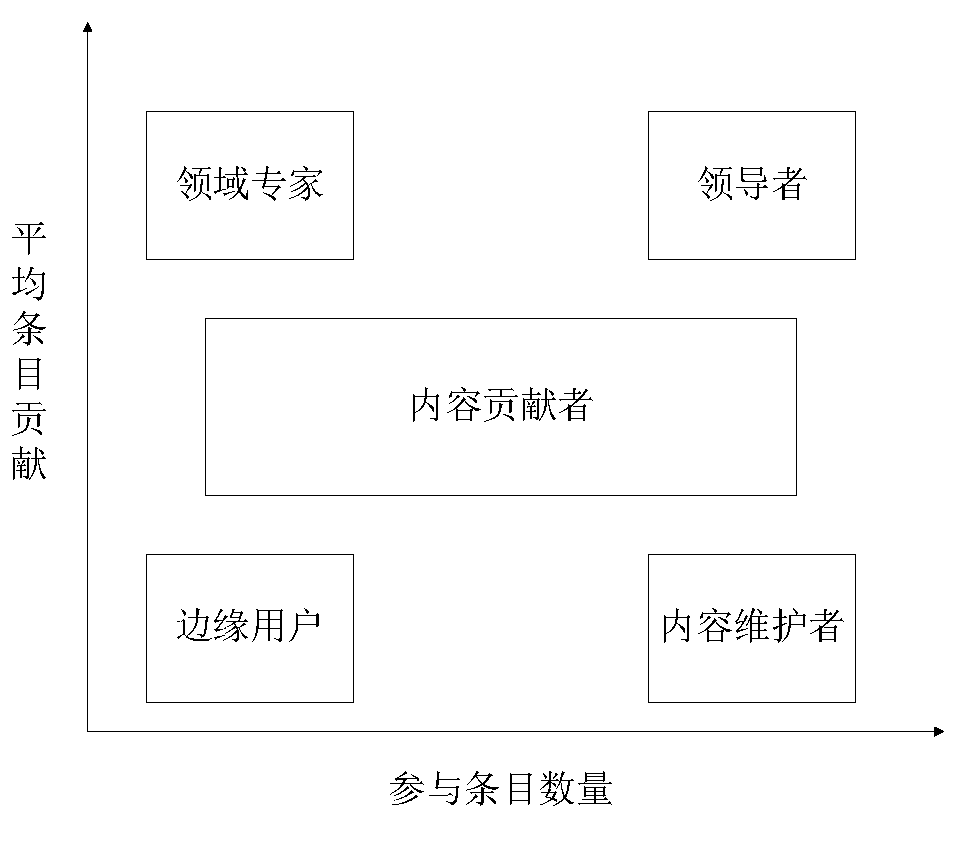
\includegraphics{user-cat.pdf}}
  \caption{\small{\textbf{不同类型的用户的特点}}}
  \label{fig:user-cat}
\end{figure}
\section{用户协同的社会网络分析}
\label{sec:social-analysis}


至此,维基百科社区中的用户依据其贡献度和参与程度两个维度共分为5个类别。
同一类型用户之间的协同以及不同类型之间的用户协同构成了社区中的所有协同
活动。用户在协同中形成了用户间的复杂网络。运用社会网络分析手段,可以更
为清晰地理解维基百科社区中用户的协同
模式。

对于复杂网络的度量,往往使用图论来研究网络属性。一个复杂网络可以表示为
$G=(V,E)$,其中$V$是网络中所有节点的集合,而$E$是节点的关联的集合。选
取不同的节点,定义不同的节点间的关联,会形成不同的网络。Capocci等将英
文维基百科中的条目作为图的节点,条目间
的关联定义为两个条目间存在引用关系,由此形成了条目网络\cite{PhysRevE.74.036116}。korfiatis等将节
点定义为内容贡献者,贡献者之间的关联定义为两个贡献者共同参与过同一条目
的编写,由此形成了贡献者网络\cite{korfiatis2006evaluating}。Jesus等同时考虑了条目和贡献者两种节点类型,提
出了二维网络,即包括条目间关联和贡献者关联的复杂网络\cite{jesus2009bipartite}。Ulrik等采取了独特
的视角构建用户的网络。用户间的关联被定义为一个用户编辑了另一用户所贡献
的内容,由此形成了区别于以往研究的社会网络\cite{1526808}。不同的复杂网络有
不同的网络特征,从不同角度揭示了维基百科社区用户协同的特点。本文将从两
个角度分析用户社会网络。一种是协同网络。网
络中的节点由用户形成的复杂网络中,用户是网络中的节点,这些节点通过某种关系而连接
起来,形成了网络中的边。如果两个用户共同参与编辑了一个条目,则认为二者
进行了知识协同,形成了网络中的关联关系。另外一种是反馈网络。在维基百科
中,用户的编辑行为获得到其他用户的反馈,如果其他用户不同意该用户所贡献
的内容,将会对其内容进行修改编辑。Ulrik等认为这揭示了用户在协同
编辑一个条目时是如何进行交互的\cite{1526808}。
由此形成的网络揭示了用户间的显式反馈,是研究用户协同行为的重要方面。

度(Degree)是复杂网络中最重要的度量之一。对于节点$i$,定义度$k_i$为与
该节点连接的其他节点的数目。在有向网络中还要进一步定义出度和入度。由于
协同关系是双相关联,即如果用户$A$与用户$B$协同一定意味着用户$B$与用户
$A$协同,因此用户网络实际上相当于无向图。在分析节点的度是主要考虑的指
标有三个:节点的平均度$\tilde{ k}=\frac{1}{N}\sum_i k_i$;节点的最大度
$k_{max}=max \  k_i$以及节点的度分布$P(k_i)$,它是节点度的概率分布函
数,表示节点$i$有$k$条边的概率。

如果在网络中不存在孤立节点,也不存在节点的自环,节点的度分布可以定义为:
\[
P(k)=\frac{\text{度为k的节点数量}}{\text{网络中节点的总数量}}
\]
显然,如果网络中有$N$个节点,则:
\[
\sum_{k=1}^{N-1}P(k)=1
\]
对于无标度网络,节点的度分布可以用一个幂函数来表示,即存在$\gamma>1,
C>0$使得
\[
P(k)= C \, k^{- \gamma}
\]
$\gamma$称为度分布指数,是描述网络特性的重要指标,随着$\gamma$增加,网
络由异质向均质过度。

集聚系数是衡量一个网络的集团化程度的重要的特征参数。在社会化网络中,如
果两个人同为一
个人的朋友,往往这两个人也是朋友。聚集系数就是为了表示网络中朋友圈的凝
聚成度,描述这种集团化现象的属性。一个节点$i$的聚集系数可以定义为于该
节点邻接的节点之间实际的连接数量同可能的最大连接数量的
比,即:$C_i=\frac{2E_i}{k_i(k_i-1)}$。其中$\frac{k_i(k_i-1)}{2}$表示
与
节点$i$邻接的节点间最大可能邻接数,而$E_i$是邻接节点间的实际连接数。这
样,通过聚集系数,可以反映不同群体间用户关联的紧密程度,从而分析其协同
模式。

\subsection{用户间协同关系分析}


领导者是所有类别中人数最少的,但是却是最为投入的群体。领导者共参与了37939
个条目的编写,平均每个人参与了622个条目。该类用户另外一个特点是:用户
参与的条目贡
献均值很高,但是贡献的方差却很大。在参与的所有条目中有$41.7\%$的条目贡献度
超过了0.8,几乎达到了单个领导者独立编写的程度;与之相对的有$39.2\%$的
条目领导者用户的贡献度
不足0.1。这个结果意味着领导者用户实际上存在着两种特征,除了自身所具有
的特征外还同时具有维护者的特征。通过进一步的分析发现,领导者用户所做的
维护工作同维护者所做的维护工作略有不同。领导者用户不是以消除文字错误、
更新信息等为目的的,而是为纠正其他用户错误的或不适当的行为为目的。由于
维基百科对用户参与的要求较高,除了必须有一定的独立撰写能力、遵从维基百
科的编写规范,还必须熟悉编写系统和标记语言的用法。对于没有经验的用户来
说很容易犯各种类型的错误。领导者于是承担起教育用户的责任,希望用户能在
参与编辑的过程中不断提升自身的水平。尽管这类用户同时存在这两种特征,但
是在接下来对用户参与知识协同活动的动机的研究中,将主要考虑领导者的特
征,而不考虑其维护者的特征。

领导者用户的最大度为42,但是平均度却只有9.2,超过一半的用户度在6以下,
说明领导者用户间很少有合作编写条目的经历,这和之前分析的领导者用户的特
征是一致的。同时,领导者的聚类系数只有0.17,远远小于整个社区的聚类系数
0.53。这说明用户之间并没有形成紧密联系的群体,一个用户也没有太多的意愿
去参与由另一个领导者主导的条目。用户间彼此的协同更多地是
在偶然的情况下发生的。

领域专家拥有和领导者类似的平均条目贡献,但是其参与条目的数量要小的多。
领域专家共计3406人,只参与了7424个条目的编写,平均每个人不到2.2个条目。
同领导者不同,领域专家的条目贡献离散程度要小的多,说明该类用户的协
同模式非常稳定:每参与到一个条目中,就尽全力把工作做好;而对于其他条目
则完全不理睬。

领域专家用户的最大度为4,平均度只有0.04,用户间的关联非常稀疏。网络的
聚集系数更是趋近于0。这类用户比领导者用户还要独立,同类用户间的协同几乎不
发生。另外,领导者和领域专家两类用户之间也鲜有协同发生。
领域专家和领导者两类用户都属于能够主导条目编写的用户,
同时有领导者和领域
专家参与编写的条目共计403个,只占领域专家参于条目总数的$5.4\%$,对于领
导者来说更是微不足道。如果把两类用户合成一类共同考察的话,在新形成的用
户网络中,节点的最大度也只有103,而平均度也只达到了0.43,仍然是非常稀
疏的连接。网络的聚集系数值为0.03,显示用户之间几乎没有任何凝聚效应。

但是,这两类用户彼此之间很少发生协同行为并不意味着这两类用户真的是特立独行
的。事实上,
在有领域专家和领导者参与的条目中,参与协同的用户数量平均为127人/条目,
远远高于社区的均值76人/条目。尽管这两类用户掌控了条目的编辑工作,但是
似乎“独裁”并未影响用户的参与程度,反倒是
由于这两类用户的积极投入,给其他用户带来了更多的参与机会去丰富内容和提
升条目质量。

内容贡献者是所有用户中参与范围最广的群体,共参与了184746个条目的编写,
几乎占整个中文维基百科条目数量的$90\%$。平均每个用户参与编写17.2个条目。巨
大的参与数量意味着该类用户同其他几类用户都具有较强的联系。其中,内容贡
献者与领导者协作参与了24954个条目,占领导者参与总量的$65.77\%$;与领域
专家协作参与了5552个条目,占领域专家参与总量的$74.79\%$。说明内容贡
献者积极地参与了这两类用户领导的条目的编写工作。另外也应该注意到,尽管
前两类两类用户都是维基百科社区的优质用户、
但是其参与的条目总数只占社区中条目总数的$21.9\%$。社区的精英并不能完成
所有的工作,还必须要依靠那些热心的普通用户配合。每个人的精力都是有限的。
对于维基百科这样完全依靠参与者在业余时间自愿投入的社区来说,明星用户永
远是少数,群体的力量才是真正可以依靠的力量。内容贡献者本身就承担了大量
的内容编写工作,是整个社区中力量最大的群体。

同领导者和领域专家不同,内容贡献者群体内部的协同非常频繁和活跃。网络节
点的最大度为7109,平均度为195,均远远高于其他两个类别。网络的聚集系数为
0.65,体现出了非常明显的聚集特征,意味着这一类用户的协同效应非常显著。
尽管他们每个人的能力都是有限的,但是他们依靠集体的
力量,相互合作,最终为社区做出自己的贡献。

维护者也是一个广泛参与知识协同的群体。该类用户共参与了143863个条目的编
写,约占条目总量的$70\%$。平均每个用户参与编辑24.5个条目。维护者与内容
贡献者的具有类似的网络特征。同上述几类用户的联系也非常紧密。其中,维护
者与领导者共同参与了21192个条目,占领导者参与总量的$55.86\%$;与领域专
家共同参与了5410个条目,占领域专家参与总量的$72.87\%$;与内容贡献者共
同参与了132539个条目,占维护者参与总量的$92.13\%$。可以看到,维护者与
社区中的主要成员关系都非常密切,尤其是和内容贡献者的联系最为紧密。

维护者群体内部的知识协同是所有类型用户中最为频繁和活跃的。其网络节点的
最大度数为5104,虽然不及内容贡献者的最大度,但是该类用户的数量只有内容
贡献者的一半,所以其平均度达到了320,为所有类别中最高。网络的聚集系数
为0.63,其聚集特征更为明显,成员之间的关系也更为密切。

边缘用户是人数最多的一类用户,但是却只参与了27732个条目的编写,平均每
人参与的条目为0.97个,是所有类型用户中最少的。边缘用户与其他类别的用户
协同则呈现明显的两极分化的特征。其与领导者共同参与了4299个条目,占边缘
用户参与总量的$15.49\%$;与领域专
家共同参与了1270个条目,占领域专家参与总量的$17.11\%$。而与之相对的,与内容贡献者共
同参与了27254个条目,占边缘用户参与总量的$98.28\%$,与维护用户共同参与
了26134个条目,占边缘用户参与总量的$94.24\%$。边缘用户几乎所有的协同都
是和内容贡献者和维护者之间发生的,而与领导者和领域专家间的协同则非常少。
这一方面是由于领导者和领域专家所参与条目的数量比较少,同时也是由于这两
类用户领导的条目质量普遍较高,并没有给边缘用户太多的参与机会。而内容贡
献者和维护者受自身条件的限制,需要更多的用户来补充完善条目内容,从而给边缘用户留下了较多参与协同的空间。

边缘用户之间基本上没有什么直接联系,只有少数人具有较高的度。最大度为
151,但是有近$1/3$的用户度为0,也就是没有和任何其他边缘用户间发生过协
同,而网络平均度为9,表明连接是非常稀疏的。边缘用户的聚类系数为0.09,
证明用户之间非常独立,没有聚集特征。

\subsection{用户间反馈关系分析}
如果两个用户$u,v$间发生过以下操作中的一种或几种,则两个用户同属于一个
反馈网络:
\begin{enumerate}
\item 用户$u$删除了用户$v$编辑的内容。
\item 用户$u$恢复了用户$v$删除的内容(该内容可能由$u,v$以外的其他用户
  编写)。
\item 用户$u$恢复了用户$v$编辑的内容(该内容可能被其他用户删除)。
\end{enumerate}
用户也可以针对自己之前编辑的内容进行以上操作,形成节点的自环。自环对于
研究用户间的反馈没有意义。在本研究中,
将忽略用户的自环。
用户间的反馈可以经由条目不同版本的比较得出。每种类型的用户均可以根据以
上定义的关联形成自己的反馈网络。该网络由特定类型的用户和所有编辑过这些
用户所贡献的内容的其他类型的用户组成。因为编辑是单向的活动,因此该网络
是有向图。

在由领导者用户生成的反馈网络中,领导者不再象在协同网络中处于中心地位。
这是由于领导者用户自身的编辑水平较高,所贡献的内容很少被其他用户所修改
或者回退。在该网络中,网络的平均度为16.37,度分布指数$\gamma$为3.41。
对于无标度网络,度分布指数一般在2--3之间,当$\gamma >3$时,网络已经不
再具有无标度属性,而是显示出随机网络的特性。用户间的关联是偶然的、随机
的。这意味着领导者用户很少受到其他用户的影响,其活动的独立性非常高。

和领导者用户类似,领域专家用户所生成的反馈网络也表现出了这种特征。网络
的平均度为14.47,度分布指数$\gamma$为3.13,同样也表现出随机网络的特征。
因此领域专家用户不会受到其他用户太大的影响,依旧保持较高的独立性。

在由内容贡献者生成的反馈网络中,内容贡献者和少量的内容维护者处于网络的
中心地位。该网络显现出比较明显的无标度特性:网络的平均度为33.41,度分
布指数$\gamma$为2.37。网络中节点度的分布极不均匀,存在大量度很小的节点
和少部分度很大的节点。内容维护者即参与到修订其他用户编辑的内容,同时自
身编辑的内容也受到其他用户的变更。内容贡献者所编写的内容越多,来自他人
的编辑就越频繁,因此内容贡献者和其他类型用户的关系非常紧密,容易受到他
人行为的影响。

内容维护者的反馈网络也是无标度网络。网络平均度为26.89,度分
布指数$\gamma$为2.29。在网络中,节点度比较大的节点既有内容维护者,也有
内容贡献者。内容维护者即频繁与其他类型的用户交互,同时也容易受到其他类
型用户活动的影响。

边缘用户的网络比较稀疏,网络的平均度只有13.84。一方面边缘用户自身的贡
献比较少,另一方面边缘用户所编写的内容质量普遍较差,容易被其他用户修改。
网络的度分
布指数$\gamma$为2.11。网络中度较高的几点大部分是内容贡献者和内容维护者。
这两类用户是编辑边缘用户贡献内容的主力,而边缘用户自己鲜有度较高的节点。由此显示边缘用户容易受到其他用
户的影响。

通过社会网络分析,本文分析了维基百科社区中5类用户的协同行为和其特征。
可以明显地看出社区中主要存在两种形式的协同:一种是以领导者或者领域专家
为主导,内容贡献者和维护者参与辅助性工作最终完成条目的编写;另一种形式是参
与编写的条目中没有真正的主导者,而是由多个内容贡献者和维护者通力合作,
利用集体的力量共同完成的。这个结果同时也回答了人们一直以来对维基百科如
何取得成功而产生的疑问:究竟是“少数人的力量”还是“多数人的智慧”。一
部分学者认为如此数量巨大的内容不可能仅仅由少数人来完成,必然是很多人齐
心协力的结果;而维基百科的创始人Jimmy Wales则以英文维基百科为例,列举
了用户参与的数据:“有$50\%$的编辑是由不到$0.7\%$的用户完成的,最活跃
的$2\%$的用户,约1400人,则贡献了总编辑数量的$73.4\%$。基于这些数据,
他认为维基百科实际上是凭借少数精英的力量发展壮大的。本文的研究结果
表明,两种协同模式的
存在使得维基百科既体现了“少数人的力量”,又体现了“多数人的智慧”。少数明
星用户是社区最积极的推动力量,并取得了非常耀眼的成就,但是这并不意味着
其他用户就处于陪衬的角色。不同类型的用户通过不同的协同模式为社区贡献力量,最终才造就了维基百科的成
功。

\section{本章小结}
\label{sec:conclusion}

本章利用上一章研究的用户贡献算法,对维基百科中的数据进行整理和分析,并
从用户贡献和用户参与程度两个维度对维基百科社区中的用户进行了分类。分类
经过调整和合并后共分为五类:领导者、领域专家、内容贡献者、内容维护者以
及边缘用户。随后分析了这五类用户的特征,并使用社会网络分析研究了不同用
户的协同模式分析结果表明,这五类用户各自都有独特的协同模式,因此其参与
协同的动机可能各不相同。在随后的章节中将分别讨论各个动机因素对每种用户
的影响,构建每类用户的动机模型。
%%% Local Variables: 
%%% mode: latex
%%% TeX-master: t
%%% End: 
